\documentclass[12pt]{article}

\usepackage[utf8]{inputenc}
\usepackage{latexsym,amsfonts,amssymb,amsthm,amsmath}
\usepackage{tikz}
\usepackage{stanli}
\usetikzlibrary{shapes,calc,through,3d,patterns}
\usetikzlibrary{arrows.meta,decorations.pathreplacing,angles,quotes}
\usepackage{multicol}
\usepackage{geometry}
\usepackage{mathtools}
\usepackage{siunitx}
\usepackage{booktabs}

\setlength{\parindent}{0in}
\setlength{\oddsidemargin}{-0.25in}
\setlength{\textwidth}{7in}
\setlength{\textheight}{9.3in}
\setlength{\topmargin}{-1in}
\setlength{\headheight}{18pt}

\newcommand\blfootnote[1]{%
    \begingroup
    \renewcommand\thefootnote{}\footnote{#1}%
    \addtocounter{footnote}{-1}%
    \endgroup
}

\definecolor{darkred}{rgb}{0.6,0,0}

\newcommand{\bolddelta}{\boldsymbol\delta}
\newcommand{\boldxi}{\boldsymbol\xi}



\begin{document}

\noindent ME473 - Dynamic finite element analysis of structures\hfill EPFL\\
Stefano Burzio \hfill 2025\\
\vspace{0.3cm}

\hspace*{\fill}\textbf{\Large Problem set 5 - solutions}\hspace*{\fill}

\hrulefill

\subsection*{Problem 1}
\noindent a)\ Degree of freedom classification:

\begin{center}
    \begin{tikzpicture}
        % Nodes
        \def\c{0.7071}
        \def\s{0.7071}
        \coordinate (1) at (0,0);
        \coordinate (2) at (2.5*\s,2.5*\c);
        \coordinate (3) at (0,5);
        %Supports 
        \point{a}{0}{5};
        \point{b}{2.5*\s}{2.5*\c};
        \support{1}{a}[-180];
        \support{1}{b}[-180];
        % Members
        \draw[ultra thick] (1) -- (2);
        \draw[ultra thick] (3) -- (1);
        \draw[thick] (1.3,0.7) circle(0.2cm);
        \node at (1.3,0.7) {1};
        \draw[thick] (-0.5,2.5) circle(0.2cm);
        \node at (-0.5,2.5) {2};
        % Points
        \node[below left=1pt,darkred] at (1) {1};
        \node[below right=1pt,darkred] at (2) {2};
        \node[below right=1pt,darkred] at (3) {3};
        % DOFs
        \draw[latex-,  thin] (-0.1,0) -- ++(-1,0) node[left] {$1$};
        \draw[latex-, thin] (0,-0.1) -- ++(0,-1) node[below] {$2$};
        \draw[-latex,  thin] (2.5*\s,2.5*\c) -- ++(1,0) node[right] {$3$};
        \draw[latex-,  thin] (2.5*\s,2.5*\c-0.1) -- ++(0,-1) node[below] {$4$};
        \draw[-latex,  thin] (3) -- ++(1,0) node[right] {$5$};
        \draw[-latex,  thin] (3) -- ++(0,1) node[above] {$6$};
        % Pins
        \draw[thick,fill=white] (3) circle (3pt);
        \draw[thick,fill=white] (2) circle (3pt);
        \draw[thick,fill=white] (1) circle (3pt);
    \end{tikzpicture}
\end{center}
\noindent % No indentation at the start
\begin{minipage}[t]{0.3\textwidth}
    % Left side content
    \begin{center}
        \begin{tabular}{c|c}
            DOF index & Description  \\
            \midrule
            1         & \( q_{1x} \) \\
            2         & \( q_{1y} \) \\
            3         & \( q_{2x} \) \\
            4         & \( q_{2y} \) \\
            5         & \( q_{3x} \) \\
            6         & \( q_{3y} \) \\
        \end{tabular}
    \end{center}
\end{minipage}
\hspace{1cm}
\begin{minipage}[t]{0.48\textwidth}
    \vspace{-1.5cm}
    % Right side content
    Each node contributes two degrees of freedom (horizontal and vertical displacements). Thus, the system has six DOFs. Nodes 2 and 3 are fully fixed, thus $q_{2x}=q_{2y}=q_{3x}=q_{3y}=0$, the only free DOFs are $1$ and $2$, the horizontal and vertical displacements of node 1.
\end{minipage}

\vspace{0.3cm}
\noindent b)\ Reduced system formulation: the full stiffness and loads vectors are respectively a $6\times 6$ matrix and a $6\times 1$ vector. However, since the unconstrained DOFs are indexed by $1$ and $2$, these are the only lines and columns we shall compute and include in the reduced stiffness matrix and applied loads vector. Bars parameters are:
\begin{center}
    \begin{tabular}{c|c|c}
        Elements & Orientations (${}^e\theta$) & Lengths (${}^e\ell$) \\
        \hline
        1        & $45^{\circ}$                & $5$ m                \\
        2        & $90^{\circ} $               & $10$ m               \\
    \end{tabular}
\end{center}
Therefore, after applying boundary conditions, the two reduced element stiffness matrices in global coordinates are:
\begin{align*}
    {}^1\mathbf{K} & =\frac{EA}{{}^1\ell}\begin{bmatrix}
                                             \cos^2({}^1\theta)               & \sin({}^1\theta)\cos({}^1\theta) \\
                                             \sin({}^1\theta)\cos({}^1\theta) & \sin^2({}^1\theta)
                                         \end{bmatrix} = \frac{EA}{10}\begin{bmatrix}
                                                                          1 & 1 \\
                                                                          1 & 1
                                                                      \end{bmatrix} \\
    {}^2\mathbf{K} & =\frac{EA}{{}^2\ell}\begin{bmatrix}
                                             \cos^2({}^2\theta)               & \sin({}^2\theta)\cos({}^2\theta) \\
                                             \sin({}^2\theta)\cos({}^2\theta) & \sin^2({}^2\theta)
                                         \end{bmatrix}=\frac{EA}{10}\begin{bmatrix}
                                                                        0 & 0 \\
                                                                        0 & 1
                                                                    \end{bmatrix}
\end{align*}
As we assemble we obtain the reduced stiffness matrix:
$$
    {}\mathbf{K}={}^1\mathbf{K}+{}^2\mathbf{K} =\frac{EA}{10}
    \begin{bmatrix} 1 & 1 \\ 1 & 2
    \end{bmatrix}.
$$
The reduced applied loads vector $\mathbf f$ can be computed directly without having to estimate the two elementary loads vectors ${}^1\mathbf f$ and ${}^2\mathbf f$. We have
$$\mathbf f= \begin{bmatrix} -25000 \\ 0
    \end{bmatrix}.$$

\vspace{0.3cm}
\noindent c)\ Displacement calculation: solving the reduced linear system
\[
    \frac{EA}{10}\begin{bmatrix} 1 & 1 \\ 1 & 2 \end{bmatrix} \begin{bmatrix} q_{1x} \\ q_{1y} \end{bmatrix} = \begin{bmatrix} -25000 \\ 0 \end{bmatrix}
\]
yields to (static) displacements for node 1:
\[
    q_{1x} = -\frac{500'000}{EA}, \quad\text{and}\quad q_{1y} = \frac{250'000}{EA}.
\]
The displacements indicate that node 1 experiences negative horizontal and positive vertical displacements; this behavior is consistent with the direction of the applied load and the geometry of the structure.

\vspace{0.3cm}
\noindent d)\ Stress evaluation: the approximated axial stress in each element is computed using the formula:
\[
    {}^e\sigma^h = \frac{E}{{}^e\ell} \begin{bmatrix} -\cos({}^e\theta) & -\sin({}^e\theta) & \cos({}^e\theta) & \sin({}^e\theta) \end{bmatrix} \begin{bmatrix}
        q_{ix} \\ q_{iy} \\ q_{jx} \\ q_{jy}
    \end{bmatrix}
\]
where we suppose that, in general, element $e$ is connected to nodes numbered as $i$ and $j$.
For element 1 ($\theta = 45^\circ$, $\ell = 5$ m):
\[
    {}^1\sigma^h = \frac{E}{5} \begin{bmatrix} -\frac{\sqrt{2}}{2} & -\frac{\sqrt{2}}{2} & \frac{\sqrt{2}}{2} & \frac{\sqrt{2}}{2} \end{bmatrix} \begin{bmatrix}
        -500'000/EA \\ 250'000/EA \\ 0 \\ 0
    \end{bmatrix} = \frac{25'000\sqrt{2}}{A}
\]
For element 2 ($\theta = 90^\circ$, $\ell = 10$ m):
\[
    {}^2\sigma^h = \frac{E}{10} \begin{bmatrix} 0 & -1 & 0 & 1 \end{bmatrix} \begin{bmatrix}
        -500'000/EA \\ 250'000/EA \\ 0 \\ 0
    \end{bmatrix} = -\frac{25'000}{A}
\]
The computed stresses indicate that element 1 experiences a tensile stress, while element 2 is under compressive stress. This is consistent with the overall structural behavior: the applied horizontal load at node 1 pulls on element 1, stretching it, while simultaneously pushing down against the vertical support, placing element 2 in compression. These stress signs reflect the internal force directions that balance the applied load and maintain equilibrium.

\subsection*{Problem 2}
The \texttt{MATLAB} code provided below solves the transient analysis of a two-dimensional steel truss using the finite element method. The approach follows standard steps in structural dynamics: material definition, finite element modeling, modal analysis, and time-domain response.

\subsubsection*{Material properties}
The code begins by defining the material properties of structural steel:

\begin{verbatim}
clear all

% E: modulus of elasticity
E = 21010^9;
% A: area of cross section
A = 6.4510-4;
% EA: axial stiffness
EA = E*A;
% rho: density
rho = 7800;
% rhoA: mass per unit length
rhoA = rho*A;
% Applied force
f = 22000;
\end{verbatim}

\subsubsection*{Geometry and mesh connectivity}
The truss geometry is defined through a node coordinate matrix and a connectivity matrix. The nodes are arranged in a simple triangular configuration, and elements are formed between nodes via the connectivity table. A plotting function \texttt{draw2Dtruss} is used to visually confirm the mesh.

\begin{verbatim}
nodesCoordinates = 6*[0 0; 0 1; 1 0];
connectivity = [1 2; 2 3; 1 3];

numberOfNodes = size(nodesCoordinates,1);
GDof = 2*numberOfNodes;

draw2Dtruss(nodesCoordinates, connectivity, ...
'LineColor', 'r', ...
'LineWidth', 2, ...
'MarkerSize', 8, ...
'ShowNodeNumbers', true);
\end{verbatim}

\subsubsection*{Global stiffness and consistent mass matrices}
The next step involves the computation of the global stiffness matrix and global consistent mass matrix using helper functions \texttt{formStiffness2Dtruss} and \texttt{formConsistentMass2Dtruss}. These matrices represent the elastic and inertial properties of the system, respectively.

\begin{verbatim}
% compute and assemble the structure stiffness matrix
stiffness = formStiffness2Dtruss(GDof, connectivity, nodesCoordinates, EA);

% compute and assemble the structure mass matrix
mass = formConsistentMass2Dtruss(GDof, connectivity, nodesCoordinates, rhoA);
\end{verbatim}

\subsubsection*{Applying boundary conditions and solving the eigenproblem}
Boundary conditions are applied by specifying the constrained degrees of freedom. Node 1 is fully fixed, and node 4 is constrained in the $y$-direction, leaving three free DOFs.

\begin{verbatim}
prescribedDof = transpose([1 2 6]);
activeDof = setdiff(transpose((1:GDof)), prescribedDof);
stiffness_freeDofs = stiffness(activeDof,activeDof);
mass_freeDofs = mass(activeDof,activeDof);

[modal_matrix,frequencies] = computeFrequenciesAndModes(GDof,prescribedDof,stiffness,
                                mass,0);
\end{verbatim}
Notice that normal modes are only relative values which may be scaled of normalized to some extent as a matter of choice. Use the following normalization convention is in force:
$$n_i=\frac{\phi_i}{\sqrt{\phi_i^T\mathbf M \phi_i}}$$
The vectors $n_i$ are referred as normalized modal vectors.

\subsubsection*{Mode normalization and orthogonality checks}
The eigenvectors computed by the \texttt{eig} function in MATLAB are not guaranteed to follow a particular normalization convention. In the context of structural dynamics, however, it is often convenient to normalize the mode shapes with respect to the mass matrix such that:
$$\boldsymbol{\Phi}^T \mathbf{M} \boldsymbol{\Phi} = \mathbf I,$$
This normalization ensures that the modal matrix $\boldsymbol\Phi$, which collects the mode shapes as columns, satisfies:
$$\boldsymbol{\Phi}^T \mathbf{K} \boldsymbol{\Phi} = \mathbf {\Lambda},$$
where $\mathbf {\Lambda}$ is the diagonal matrix of eigenvalues $\lambda_i=\omega_i^2$. The following code performs this mass-normalization of the mode shapes and verifies the orthogonality relations with respect to both the mass and stiffness matrices. These checks confirm that the system of modal coordinates is decoupled and can be treated as independent single-degree-of-freedom systems during transient analysis.

\begin{verbatim}
modes_normalized = zeros(size(modal_matrix));
for modeNumber = 1:size(modal_matrix,2)
norm = sqrt(transpose(modal_matrix(:,modeNumber)) * mass_freeDofs * 
        modal_matrix(:,modeNumber));
modes_normalized(:,modeNumber) = 1 / norm * modal_matrix(:,modeNumber);
end

% Check orthogonality with respect to stiffness matrix
transpose(modal_matrix) * stiffness_freeDofs * modal_matrix
frequencies.^2

% Check orthogonality with respect to mass matrix
transpose(modal_matrix) * mass_freeDofs * modal_matrix
\end{verbatim}

\subsubsection*{Transient analysis}
The transient response of the structure is evaluated in modal coordinates using the modal superposition method. The transformation $\mathbf{q}(t) = \boldsymbol{\Phi} \, \mathbf{z}(t)$ yields the modal force vector, which drives each of the uncoupled second-order ordinary differential equations (ODEs) of the form:
$$\mathbf I\ddot{\mathbf z}(t)+\mathbf \Lambda\mathbf z(t)=\mathbf p$$
where $\mathbf \Lambda=\text{diag}(\lambda_1^2,\lambda_2^2,\lambda_3^2)$ and the modal force is
$$\mathbf p=\boldsymbol{\Phi}^T \mathbf{f}.$$
The modal equations are given in components by
$$\ddot z_i(t)+\omega_i^2 z_i(t)=p_i.$$
Hence the uncoupled system of equations is
$$\begin{cases}\ddot z_1(t)+506400\, z_1(t)=p_1 \\ \ddot z_2(t)+224360\, z_2(t)=p_2 \\ \ddot z_3(t)+324770\, z_3(t)=p_3\end{cases}$$
where
\begin{verbatim}
p = transpose(modal_matrix) * [f; 0; 0];
\end{verbatim}
The solution of the above equations for zero initial conditions $\mathbf z(0)=\dot{\mathbf z}(0)=0$ is given by
$$\begin{cases}
        z_1(t) = \frac{p_1}{\omega_1^2}(1 - \cos\big(\omega_1^2 t)\big) \\
        z_2(t) = \frac{p_2}{\omega_3^2}(1 - \cos\big(\omega_2^2 t)\big) \\
        z_3(t) = \frac{p_3}{\omega_2^2}(1 - \cos\big(\omega_3^2 t)\big)
    \end{cases}$$

\begin{verbatim}
syms t
z = vpa(p ./ frequencies.^2 .* (1 - cos(frequencies.^2 * t)),3);
q = vpa(modal_matrix * z, 3)
\end{verbatim}

The time response at the nodal coordinates is calculated from $\mathbf{q}(t)={\Phi}\, \mathbf z(t)$.

\subsubsection*{Plotting the time responses}
We now compute and plot the time responses $q_1(t)$, $q_2(t)$, and $q_3(t)$ over a given time interval.

\begin{verbatim}
% Define time vector
t_vals = linspace(0, 0.1, 1000);
q_time = zeros(3, length(t_vals));

for i = 1:length(t_vals)
z_t = p ./ frequencies.^2 .* (1 - cos(frequencies .* t_vals(i)));
q_time(:, i) = modal_matrix * z_t;
end

% Plot q_1(t)
figure;
plot(t_vals, q_time(1, :), 'LineWidth', 2);
xlabel('Time (s)'); ylabel('Displacement q_1(t) [m]');
title('Time Response of q_1(t)'); grid on;
\end{verbatim}

\begin{verbatim}
% Plot q_2(t)
figure;
plot(t_vals, q_time(2, :), 'LineWidth', 2);
xlabel('Time (s)'); ylabel('Displacement q_2(t) [m]');
title('Time Response of q_2(t)'); grid on;
\end{verbatim}

\begin{verbatim}
% Plot q_3(t)
figure;
plot(t_vals, q_time(3, :), 'LineWidth', 2);
xlabel('Time (s)'); ylabel('Displacement q_3(t) [m]');
title('Time Response of q_3(t)'); grid on;
\end{verbatim}

\begin{center}
    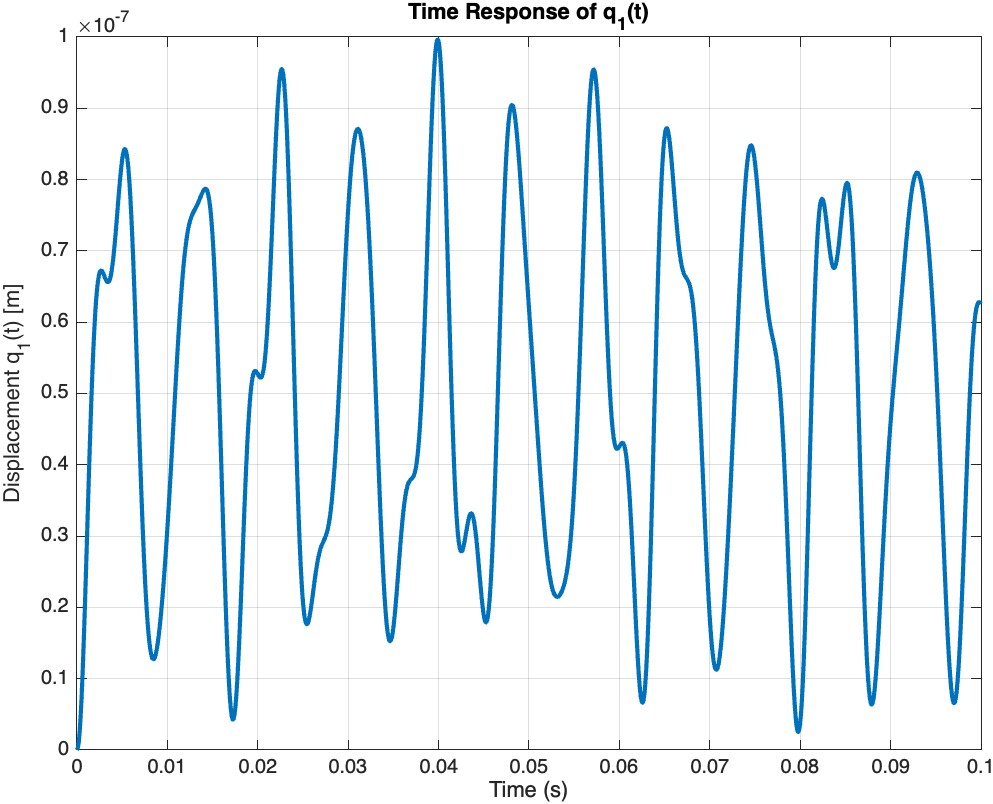
\includegraphics[width=5cm]{../images/truss2dq1.jpg}
    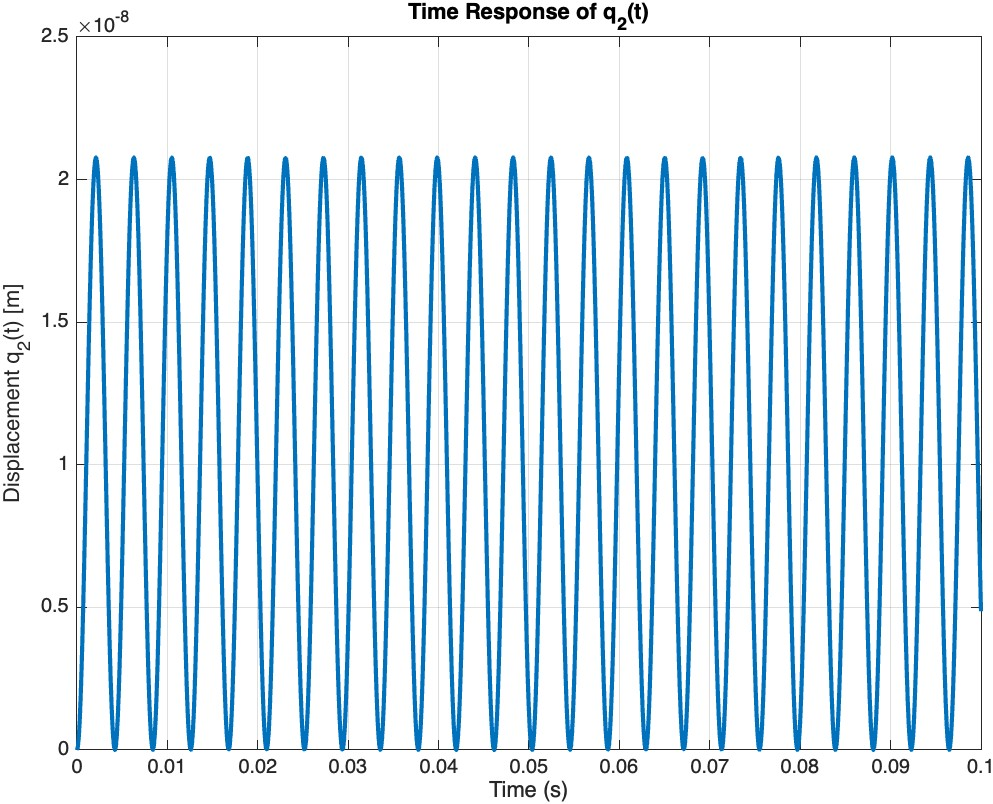
\includegraphics[width=5cm]{../images/truss2dq2.jpg}
    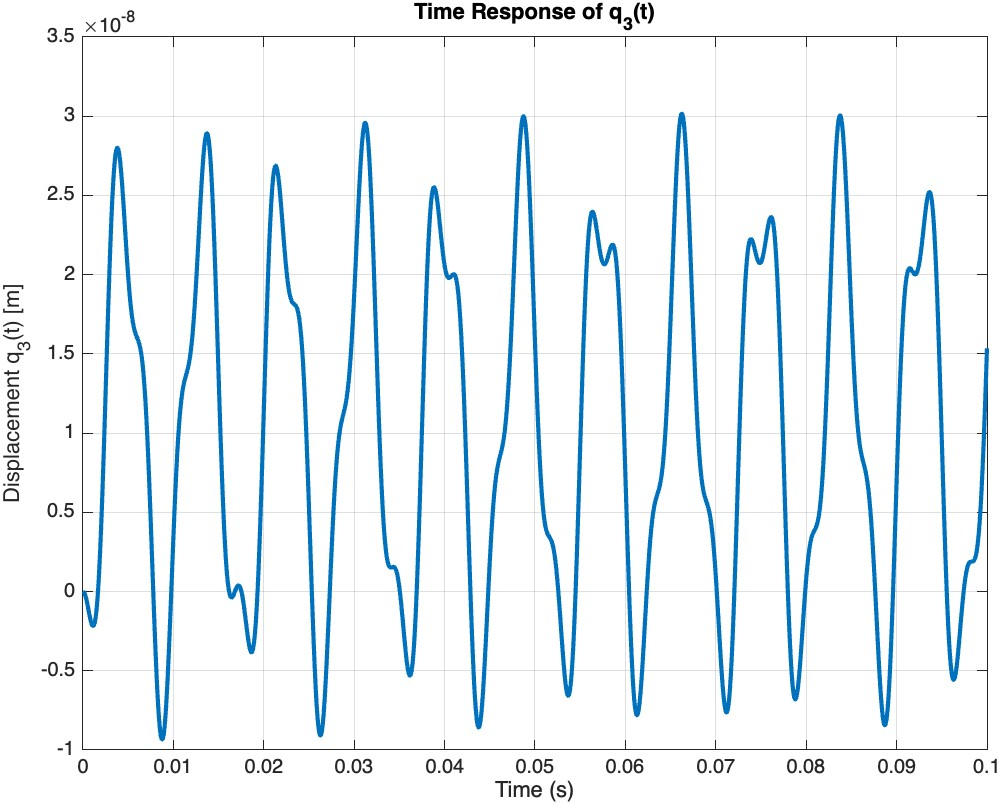
\includegraphics[width=5cm]{../images/truss2dq3.jpg}
\end{center}
\end{document}